\begin{figure}[h]
\centering
\tikzset{every picture/.style={line width=0.75pt}} %set default line width to 0.75pt        

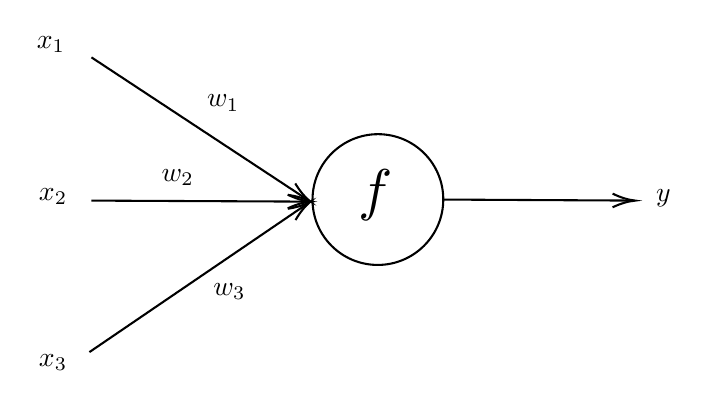
\begin{tikzpicture}[x=0.75pt,y=0.75pt,yscale=-1,xscale=1]
%uncomment if require: \path (0,194); %set diagram left start at 0, and has height of 194

%Shape: Circle [id:dp058244464473876545] 
\draw   (144.99,88.5) .. controls (145.03,71.1) and (159.17,57) .. (176.57,57) .. controls (193.97,57) and (208.03,71.1) .. (207.99,88.5) .. controls (207.94,105.9) and (193.8,120) .. (176.41,120) .. controls (159.01,120) and (144.94,105.9) .. (144.99,88.5) -- cycle ;
%Straight Lines [id:da46924522998984264] 
\draw    (38.5,89) -- (141.99,89.49) ;
\draw [shift={(143.99,89.5)}, rotate = 180.27] [color={rgb, 255:red, 0; green, 0; blue, 0 }  ][line width=0.75]    (10.93,-3.29) .. controls (6.95,-1.4) and (3.31,-0.3) .. (0,0) .. controls (3.31,0.3) and (6.95,1.4) .. (10.93,3.29)   ;

%Straight Lines [id:da764532034401557] 
\draw    (38.5,20) -- (142.32,88.4) ;
\draw [shift={(143.99,89.5)}, rotate = 213.38] [color={rgb, 255:red, 0; green, 0; blue, 0 }  ][line width=0.75]    (10.93,-3.29) .. controls (6.95,-1.4) and (3.31,-0.3) .. (0,0) .. controls (3.31,0.3) and (6.95,1.4) .. (10.93,3.29)   ;

%Straight Lines [id:da33196562179949296] 
\draw    (207.99,88.5) -- (298.5,88.99) ;
\draw [shift={(300.5,89)}, rotate = 180.31] [color={rgb, 255:red, 0; green, 0; blue, 0 }  ][line width=0.75]    (10.93,-3.29) .. controls (6.95,-1.4) and (3.31,-0.3) .. (0,0) .. controls (3.31,0.3) and (6.95,1.4) .. (10.93,3.29)   ;

%Straight Lines [id:da4624390017909269] 
\draw    (37.5,162) -- (142.33,90.63) ;
\draw [shift={(143.99,89.5)}, rotate = 505.75] [color={rgb, 255:red, 0; green, 0; blue, 0 }  ][line width=0.75]    (10.93,-3.29) .. controls (6.95,-1.4) and (3.31,-0.3) .. (0,0) .. controls (3.31,0.3) and (6.95,1.4) .. (10.93,3.29)   ;


% Text Node
\draw (102,42) node  [align=left] {$w_1$};
% Text Node
\draw (175.49,86.5) node [scale=2.074]  {${\displaystyle f}$};
% Text Node
\draw (80,78) node  [align=left] {$w_2$};
% Text Node
\draw (105,133) node  [align=left] {$w_3$};
% Text Node
\draw (19,14) node  [align=left] {$x_1$};
% Text Node
\draw (20,87) node  [align=left] {$x_2$};
% Text Node
\draw (20,167) node  [align=left] {$x_3$};
% Text Node
\draw (314,88) node  [align=left] {$y$};

\end{tikzpicture}
\caption[Esquema de una neurona en una red neuronal artificial.]{Esquema de una neurona en una red neuronal artificial. En ella, $x_i$ son las entradas de la neurona, $w_i$ son los \textit{pesos} para cada entrada, $f$ es la función que aplica la neurona sobre las \textit{entradas ponderadas} e $y$ es la salida de la neurona.
\source{Elaboración propia.}} 
\label{fig:neur}
\end{figure}